% Lorentz.tex      pdflatex ZhCvGo15
% Diffuse globally, compute locally: a cyclist tale
% Tingnan Zhang, Daniel I. Goldman and Predrag Cvitanovi\'c

%\section{Diffusion in periodic arrays}
%\label{s-Lorentz}

\begin{figure}[htbp]
	\begin{center}
    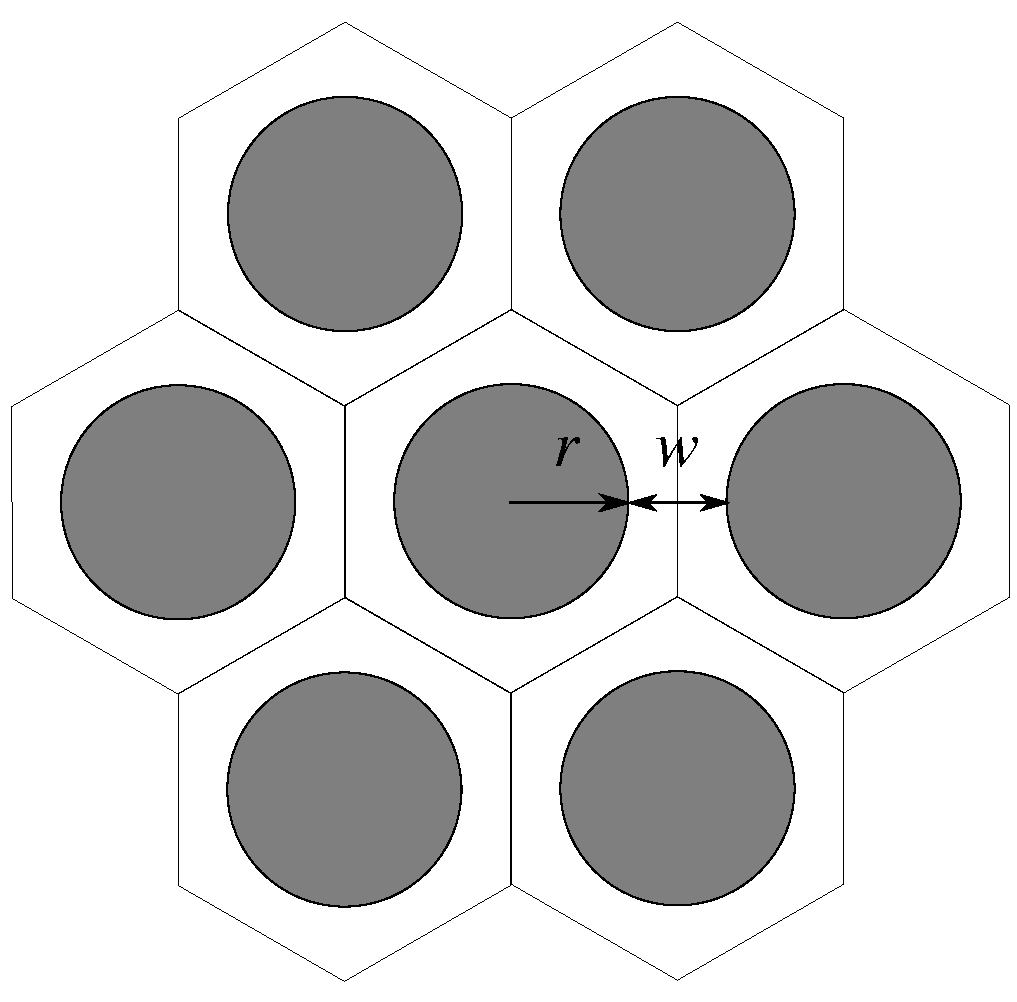
\includegraphics[width=0.25\textwidth]{diffuseLorentzGasParams}
	\end{center}
	\caption[]{\label{fig-LorentzGasParams}
    An elementary cell and its six nearest neighbor translations. The ratio of
    distance $w$ between the nearest pair of disks to the disk radius $r$
    determines the dynamical properties in the system. The transition
    between the finite and the infinite horizon is controlled by the
    ratio of $w/r$: the horizon is finite for $w/r < 4/\sqrt{3}-2
    =0.3094\cdots$.
	}
\end{figure}

Most of the periodic Lorentz gas literature, such as Bunimovich and
Sinai\rf{BunSin81}, is focused on the symmetries under discrete
translations of periodic tilings of the plane, usually defined by a
parallelepipedal ``primitive unit cell''
(also called ``fundamental domain'' in literature; here that term will
be reserved for the smallest tile that tiles the hexagon)
spanned by a pair of vectors
$\textbf{e}_1,\textbf{e}_2$, such that the center of every disk is
labeled by a pair of integers
$\hn=(m,n)=m\,\textbf{e}_1+n\,\textbf{e}_2$.
However, for a triangular periodic Lorentz gas the full symmetry group is
the space group $p6mm$ (see \refref{Cotton08chp11} for a discussion of the
geometry of space groups), and the natural tiling is in terms of the
hexagon centered on the scattering disk (``Wigner-Seitz cell'', ``Voronoi
cell''),  see \reffig{fig-LorentzGasParams}.
The full, infinite {\statesp} $\hM$ (\ie, both spatial coordinates and
momenta) then has a periodic tiling by compact \statesp\ tiles
\[ %beq
\hM=\bigcup_{ \hn \in T} \pS_{\hn},
\] %eeq
obtained by all {\em translations} a \statesp\ tile $\pS=\pS_{0}$, which
we here refer to as the {\em elementary cell}, with $T$ the abelian group
of lattice translations.

Furthermore, space group $p6mm$ has a point subgroup $\Zn{6v}=\Dn{6}$,
because the hexagonal elementary cell itself can be tiled by 12
triangular tiles,
\[ %beq
\pS=\bigcup_{\LieEl \in \Dn{6}} \tM_\LieEl,
\] %eeq
as in \reffig{fig-schrieberFig12}\,(a), upper left. We pick one of these
compact \statesp s, and refer to it as the
\emph{fundamental domain} $\tM=\tM_e$. The fundamental domain tiles the
full hexagon by its 11 copies obtained by application of the \Dn{6} point
group actions, rotations around the center or reflections across symmetry
lines. The translations then tile the entire plane.

\begin{figure}[htbp]
  \begin{center}
    (a)\;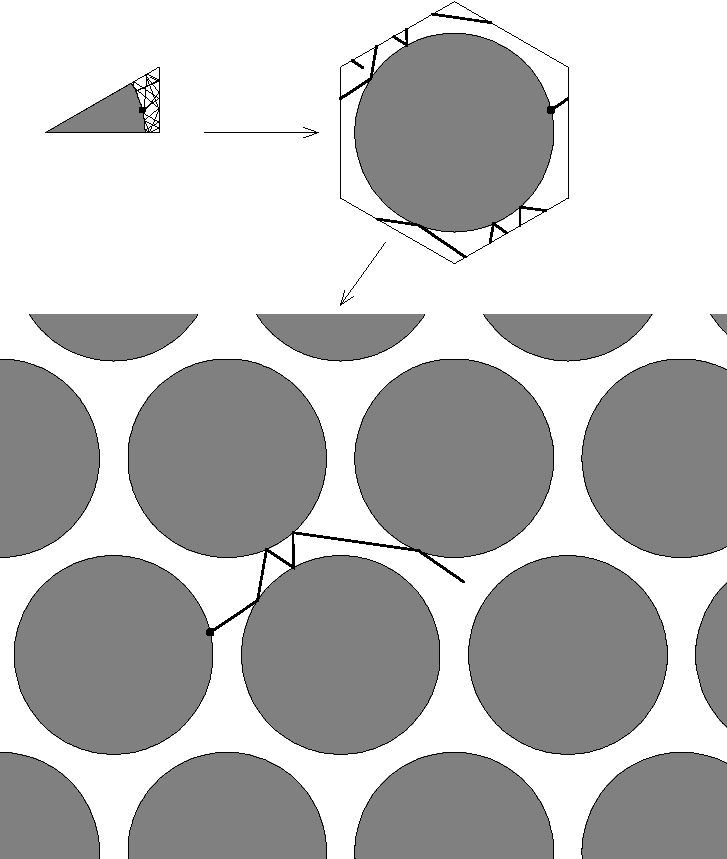
\includegraphics[width=0.43\textwidth]{diffuseSchreiberFig1}
    (b)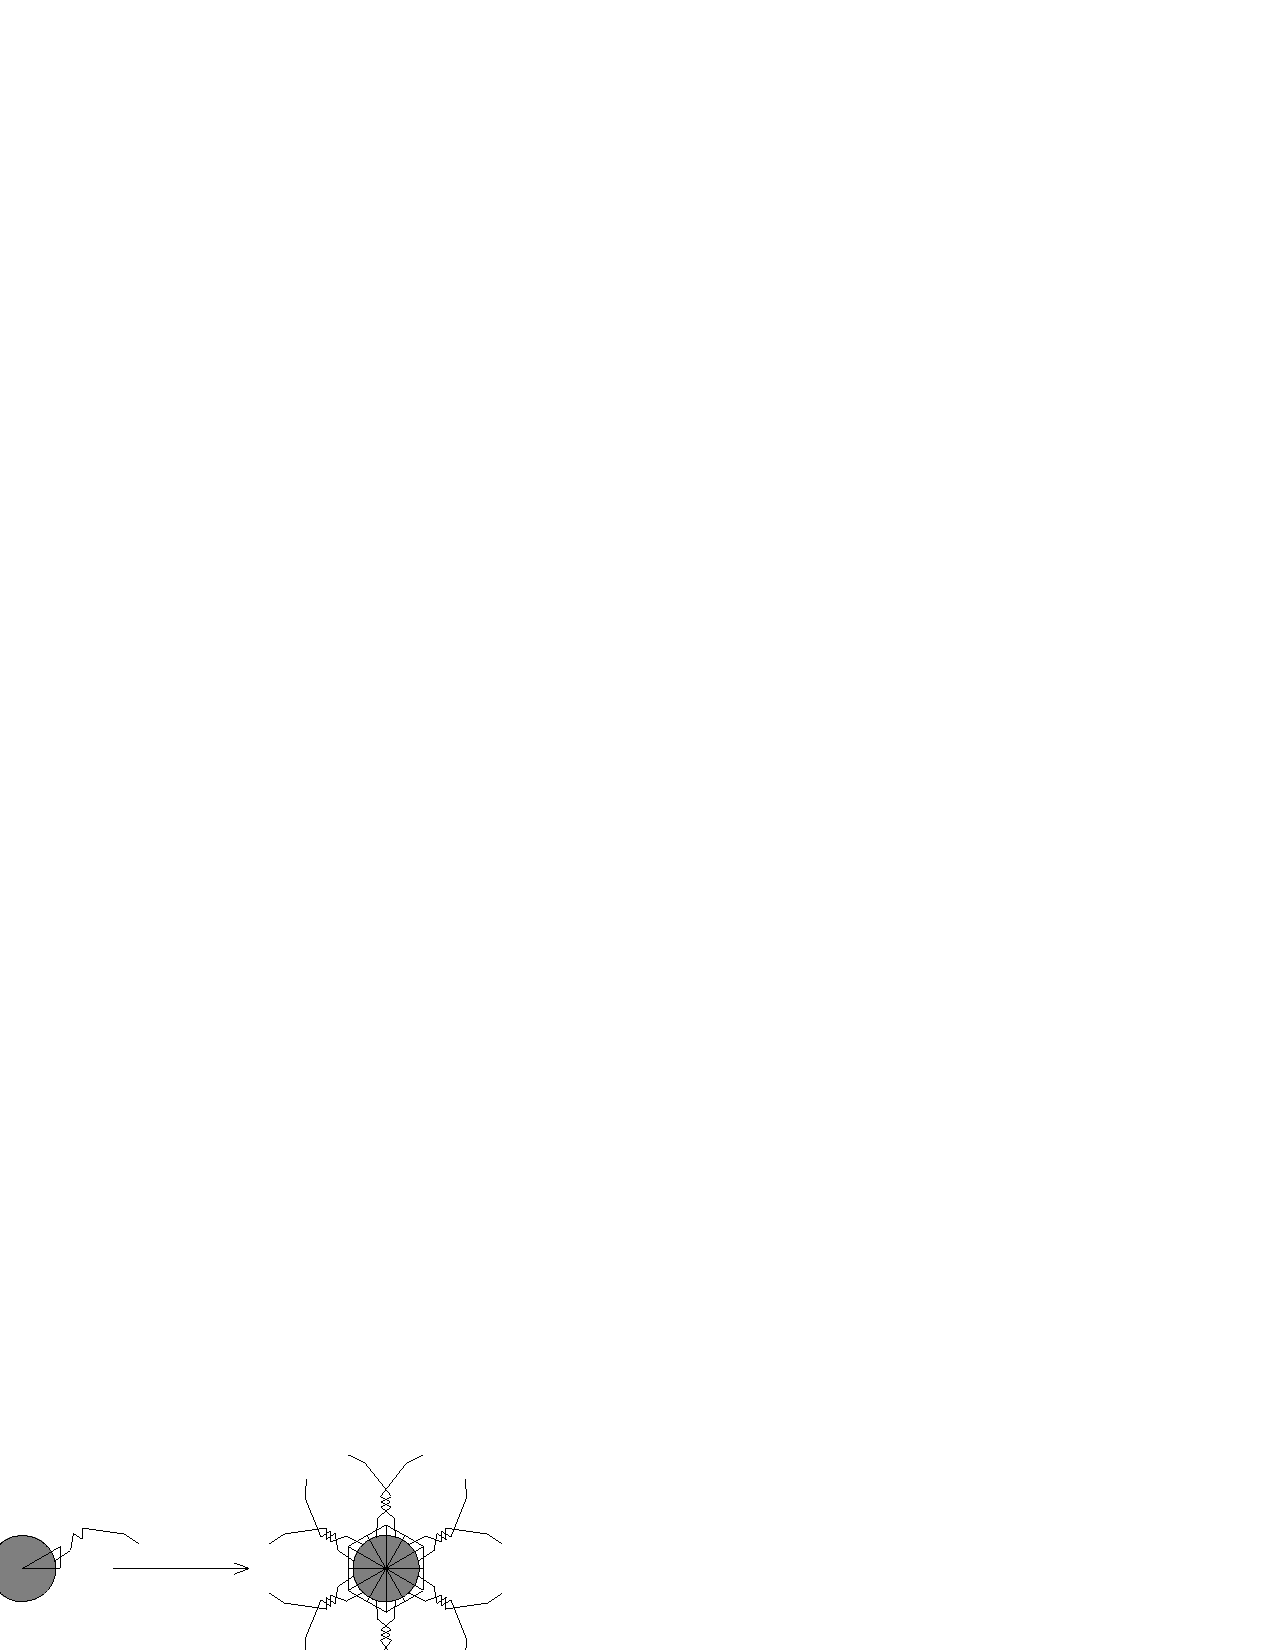
\includegraphics[width=0.45\textwidth]{diffuseSchreiberFig2}
  \end{center}
  \caption[]{\label{fig-schrieberFig12}
  (a) Motion in the fundamental domain $\tM$ (top left),
      the elementary cell $\pS$ (top right), and
      the full {\statesp} $\hM$ (bottom).
  (b) The above trajectory unwrapped in the full space and its 11 copies
    obtained by applying the twelve \Dn{6} point group actions to it (from
    \refref{CGS92}).
  }
\end{figure}


As we will work with three kinds of \statesp s,
throughout the text we will repeatedly use tildes
($\tilde{\quad}$), nothings and hats ($\hat{\quad}$) atop symbols to
distinguish dynamical quantities in the fundamental domain, elementary
cell and full {\statesp}, respectively:
\bea
&\tilde{\ }& \qquad
    \mbox{fundamental domain}\;\tM, \mbox{triangle in \reffig{fig-schrieberFig12}}
        \continue
&{\scriptstyle [nothing]}& \qquad
    \mbox{elementary cell}\;\pS, \mbox{hexagon in \reffig{fig-schrieberFig12}}
        \continue
&\hat{\ }& \qquad
    \mbox{full {\statesp}}\;\hM, \mbox{lattice in \reffig{fig-schrieberFig12}}
\label{atops}
\eea
The dynamics can be restricted to the elementary cell by imposing
periodic boundary conditions: whenever the particle leaves across the
edge of the hexagonal cell, it reenters through the opposite
edge. The corresponding discrete translation $\hn$ plays a dual role:
it is recorded in order (i)
that the full \statesp\ trajectory can be reconstructed from the
trajectory confined to the elementary cell, and (ii) to help us
construct a symbolic dynamics, see \refsect{s-elemCell}.  Let
$\hx(t)\,=\,\hflow{t}{\hx_0}$ denote the point in the full \statesp\
$\hM$ reached by the flow in time $t$. $x(t)\,=\,\flow{t}{\xInit}$
denotes the corresponding flow in the elementary cell; the two are
related by
\beq
\hn_t(\xInit)=\hflow{t}{\xInit} - \flow{t}{\xInit} \in T
\,,
\ee{l-diff-hatn1}
the discrete translation of the endpoint of the global trajectory into
the elementary cell $\pS$.
We will show  in \refsect{s-POT} that for the dynamics in the elementary
cell, the full \statesp\ displacement accrued along an elementary cell
\po\ is one-to-one and independent of the starting point.

The elementary cell dynamics can be restricted to dynamics in the
fundamental domain by applying a reflection whenever the trajectory
crosses one of the three edges of the triangle, as will be discussed in
detail in \refsect{s-FundTranslation}. We denote the quantity
$\tx(t)\,=\,\tflow{t}{\tx}$ as the flow in the fundamental domain $\tM$.
$\tflow{t}{\tx}$ is related to $\flow{t}{\tx}$ by a point group symmetry
$g \in \Dn{6}$ which maps $\tx(t)\in\tM$ to ${x}(t) \in {\pS}$.

Thus any full \statesp\ trajectory $\hx(t)$ can be uniquely reduced to
its fundamental domain counterpart $\tx(t)$. This eliminates redundancies
purely due to symmetries, and renders computations carried out in the
fundamental domain easier, with significantly faster convergence. The
reverse process, however, is always one-to-many, as illustrated by
\reffig{fig-schrieberFig12}\,(b).
As the fundamental domain does not have
the concept of absolute orientation, a single unwrapped trajectory may
have up to 11 full \statesp\ copies, with 12 orientations in all. Even worse,
depending on where we start to unwrap the trajectory, the full \statesp\
trajectories can be of completely different shapes, and, the global distance
$ \hf^{r \period{\tilde{p}}} (\tx{\tpk}) - \tx{\tpk} $,
$\tx{\tpk} \in \tp$,
% $ \hn_{r |\t p|}(\tx{\tpk}) $
depends on the starting cycle point if
$\tp$ is only a segment of the global cycle $p$. An
example is the full \statesp\ diamond-shaped 4-cycle of \reffig{schreiberFig3}; %Fig.~3;
depending whether one starts at $\tx_1$ or $\tx_2$ on the
corresponding fundamental domain 2-cycle, the global
distance covered in time $\period{\tilde{p}}$ is either the short or the
long diagonal.

%%%%%%%%%%%%%%\item[Figure 4]%%%%%%%%%%%%%%%%%%%%%%%%%%%%%%%%%%%%%%%%%%
\begin{figure}
\begin{center}
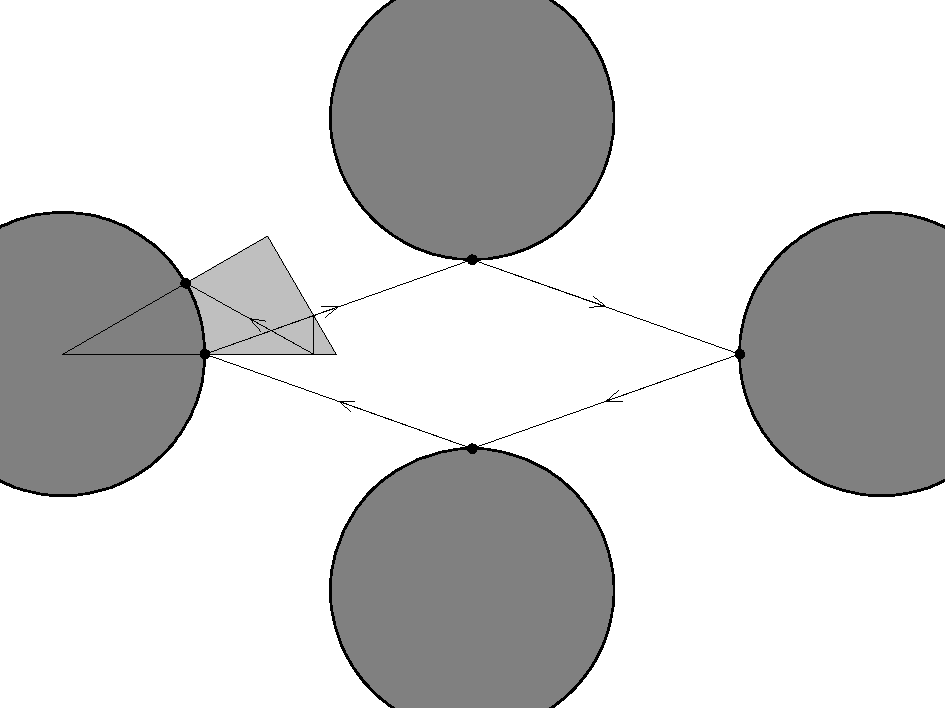
\includegraphics[width=0.45\textwidth]{diffuseSchreiberFig3}
\end{center}
\caption{
The upper row shows the case when the preceding
segment has been a short one,
the lower row the case when it has been a long one.
\PCedit{[Eckmann\rf{LorentzDiff} Fig.~3. Remember to include
schreiberFig3.tex]}
    }
\label{schreiberFig3}
\end{figure}
%%%%%%%%%%%%%%%%%%%%%%%%%%%%%%%%%%%%%%%%%%%%%%%%%%%%%%%%%%%%%%%%%%%%%%%%


How to deal with such consequences of the non-commutativity of
translations and rotations is the main thrust of this paper.

        \ifboyscout
\subsection{Brillouin zone}

    \PC{2015-10-21}
    {text from Cvitanovi\'c,  Eckmann, and Gaspard\rf{LorentzDiff}.
    Will probably give up on all of it, except for \reffig{schreiberFig3}
    or an equivalent.}
The lattice symmetry of the Lorentz billiard has important consequence on
the properties of the function $Q(\beta)$ are best illustrated by
introducing its analytic continuation at $\beta = i k$.  The function
$F(k)=Q(ik)$ is the rate associated with the incoherent scattering
function $\langle \exp i k \cdot (\hat x_t - x) \rangle_M$ considered in
light or neutron scattering experiments in liquids, in particular, by Van
Hove\rf{BoonYip80,VanHove54}. The vector $k$ is interpreted as the
wavenumber of the hydrodynamic modes of diffusion which we also find in
the Lorentz gas.  The function $F(k)$ turns out to be a dispersion
relation since $F(k)=-D k^2 + {\cal O}(k^4)$ in an isotropic diffusive
system.  The isotropy of a liquid implies that the dispersion relation
only depends on the amplitude $\vert k\vert$ of the wavenumber.

On the other hand, the lattice symmetry of the Lorentz gas
imposes special restrictions on the properties of the dispersion relation
$F(k)$ and on the values taken by the wavenumber.  The classical
problem of deterministic diffusion is similar to the quantum motion of a particle in a
periodic potential.  Hence, the wavenumber takes its values in the
Brillouin zone\rf{BoSmWi36,Harrison70}.  A mode of diffusion is associated with each value of
the wavenumber $k$ so that the direction of $k$ is privileged in the
system.  As a consequence, the symmetry of the lattice is reduced by the choice
of $k$.  This symmetry reduction is formalized by the concept of little group
associated with the wavenumber $k$, which is the subgroup of the lattice point
group leaving invariant the vector $k$.  For most values of $k$ inside the
Brillouin zone, the little group is trivial because it contains only the
identity.  However, the little group is larger when the wavenumber belongs to
special symmetry lines or symmetry points in the Brillouin zone.  In particular,
the little group coincides with the full point group when $k=0$.

In triangular and square lattices the diffusion is isotropic, but the
full function $Q(\beta)$ contains more information on the lattice
symmetry than the diffusion matrix of the second derivatives of
$Q(\beta)$. The behavior of the function $Q(\beta_x, \beta_y)$ away from
$\beta=0$ is discussed in \refref{Gaspard92a}.
    \PC{2015-12-03}{
    Lattice gases literature (Hasslacher, Frisch?) has a reference to a formula
    in Landau-Lifshitz that shows triangular lattice is isotropic - try to
    re-find this.

    ``The number of independent elastic constants is determined by the
    dimensionality and rotational symmetry of the lattice in question.  For
    example, in two dimensions, square lattices have three independent elastic
    constants, and triangular lattices are ``elastically isotropic'' (i.e.,
    elastic properties are independent of direction) and thus have only
    two\rf{Landau70}.''

    ``the  triangular  lattice  elastic  energy  is  fully  isotropic,
    i.e.  invariant under  all  rotations\rf{Landau70}''
    }

Compared to earlier literature\rf{CvitaEckardt,robb}, the new feature of the
problem at hand is use of vector-valued functions. The arbitrary vector
$\beta$ is only a device for generating moments~--~the moments themselves
are invariant under discrete symmetries, but it can be interpreted in
terms of the wavenumber of the hydrodynamic modes of diffusion.

    \fi % end         \ifboyscout
